\documentclass{beamer}
\usepackage[utf8]{inputenc}
\usetheme{Berlin}
%\usepackage{ressource}
\setbeamerfont{caption}{size=\footnotesize}

\title{Représentation probabiliste d’un parcours de navigation dans un corpus documentaire}
\subtitle{Soutenance PFE}
\author{LAINE Bastien}
\institute{Génie Mathématique | INSA Rouen}

\begin{document}
    \begin{frame}
        \titlepage{}
    \end{frame}

    \section*{Sommaire}

    \begin{frame}
        \tableofcontents[hideallsubsections]
    \end{frame}

    \section{Introduction}
        \begin{frame}
        \end{frame}

    \section{État de l'art}
        \subsection{État de l'art}
            \begin{frame}
            \end{frame}

    \section{Versions}
        \subsection{v1 - POC}
            \begin{frame}
                \frametitle{Problématiques}
                Version "Proof Of Concept"
                \begin{itemize}
                    \pause
                    \item Comment modéliser les parcours d'un utilisateur?
                    \pause
                    \item Comment prédire les documents suivants?
                \end{itemize}
            \end{frame}
            \begin{frame}
                \frametitle{Chaîne de Markov}
                Qu'est-ce que sont les chaînes de Markov?
                \pause
                \begin{block}{Description}
                    Graphe orienté dont les arêtes porte la probabilité de passage d'un nœud (=Ensemble d'états) à un autre.
                \end{block}
                \pause
                \begin{block}{Markov appliqué aux documents}
                    Dans notre cas:
                    \begin{itemize}
                        \item Les \textbf{séquences de documents} représentent les \textbf{nœuds}.
                        \item Les \textbf{probabilités de séquence suivante} représentent les \textbf{arêtes}.
                    \end{itemize}
                \end{block}
            \end{frame}
            \begin{frame}
                \frametitle{Exemples de chaîne de Markov}
                \pause
                \begin{exampleblock}{Markov d'ordre 1}
                    \begin{center}
                        \includegraphics[scale=0.5]{graph/Markov1.png}
                    \end{center}
                \end{exampleblock}
                \pause
                \begin{exampleblock}{Markov d'ordre 3}
                    \begin{center}
                        \includegraphics[scale=0.3]{graph/Markov3.png}
                    \end{center}
                \end{exampleblock}
            \end{frame}
            \begin{frame}
                \frametitle{Quelle(s) chaîne(s) considérer?}
                Quelles sont les limites qu'il faut s'imposer?
                \begin{itemize}
                    \pause[2]
                    \item Combien de Markov? \pause[3] $\Rightarrow$ \textbf{All-k}$^{th}$\textbf{-Markov}
                    \pause[4]
                    \item Ordre de Markov maximal? \pause[6] $\Rightarrow$ \textbf{Ordre 4}
                    \pause[5]
                \end{itemize}
                \begin{exampleblock}{NLP}
                    \begin{center}
                        \includegraphics[scale=0.35]{graph/NLP.png}
                    \end{center}
                \end{exampleblock}
            \end{frame}
            \begin{frame}
                \frametitle{Implémentation}
                Spécificités:
                \begin{itemize}
                    \pause
                    \item Langage: \pause C++
                    \pause
                    \item Stockage: \pause Manuel
                    \pause
                    \item Utilisation: \pause Invite de commandes/Script
                \end{itemize}
            \end{frame}
            \begin{frame}
                \frametitle{Implémentation}
                \begin{block}{Diagramme de classes}
                    \begin{center}
                        \only<1>{\includegraphics[scale=0.2]{graph/v1class.png}}
                        \pause[2]
                        \only<2>{\includegraphics[scale=0.5]{graph/v1classneat.png}}
                    \end{center}
                \end{block}
            \end{frame}
            \begin{frame}
                \frametitle{Démonstration}
                \begin{center}
                    Démonstration
                \end{center}
            \end{frame}
        \subsection{v2 Multi-Utilisateur}
            \begin{frame}
                \frametitle{Problématiques}
                Version Multi-Utilisateur
                \pause
                \begin{itemize}
                    \item Comment grouper les parcours de plusieurs utilisateurs?
                    \pause
                    \item Comment prédire les documents suivants à partir des parcours de plusieurs utilisateurs?
                    \pause
                    \item Comment grouper efficacement plusieurs utilisateurs?
                    \pause
                    \item Comment rendre l'application plus "interfacable"?
                \end{itemize}
            \end{frame}
            \begin{frame}
                \frametitle{Union de Markov}
                Comment joindre plusieurs Markov de même ordre?
                \pause[2]
                \begin{columns}[t]
                    \begin{column}{3cm}
                        \begin{exampleblock}{User 1}
                            \begin{center}
                                \includegraphics[scale=0.3]{graph/mergeUser1.png}
                            \end{center}
                        \end{exampleblock}
                    \end{column}
                    \begin{column}{3cm}
                        \begin{exampleblock}{User 2}
                            \begin{center}
                                \includegraphics[scale=0.3]{graph/mergeUser2.png}
                            \end{center}
                        \end{exampleblock}
                    \end{column}
                    \pause[3]
                    \begin{column}{3cm}
                        \begin{exampleblock}{Union}
                            \begin{center}
                                \only<3>{\includegraphics[scale=0.3]{graph/mergeUsers.png}}
                                \pause[4]
                                \only<4>{\includegraphics[scale=0.25]{graph/mergeUsersFix.png}}
                            \end{center}
                        \end{exampleblock}
                    \end{column}
                \end{columns}
            \end{frame}
            \begin{frame}
                \frametitle{Union de Markov}
                Une autre possibilité gardant les probabilités. \pause[5] \textbf{Plus claire, mais moins efficace}
                \pause[2]
                \begin{columns}[t]
                    \begin{column}{3cm}
                        \begin{exampleblock}{User 1}
                            \begin{center}
                                \includegraphics[scale=0.25]{graph/wrongMergeUser1.png}
                            \end{center}
                        \end{exampleblock}
                    \end{column}
                    \begin{column}{3cm}
                        \begin{exampleblock}{User 2}
                            \begin{center}
                                \includegraphics[scale=0.25]{graph/wrongMergeUser2.png}
                            \end{center}
                        \end{exampleblock}
                    \end{column}
                    \pause[3]
                    \begin{column}{3cm}
                        \begin{exampleblock}{Union}
                            \begin{center}
                                \only<3>{\includegraphics[scale=0.25]{graph/wrongMergeUsers.png}}
                                \pause[4]
                                \only<4,5>{\includegraphics[scale=0.25]{graph/wrongMergeUsersFix.png}}
                            \end{center}
                        \end{exampleblock}
                    \end{column}
                \end{columns}
            \end{frame}
            \begin{frame}
                \frametitle{Groupement d'utilisateur}
                Quel est le but du groupement d'utilisateurs?
                \pause
                \begin{itemize}
                    \item Créer des groupes d'utilisateurs partagent les mêmes intérêts
                    \pause
                    \item Réunir les utilisateurs \textbf{proches} en terme d'intérêt
                    \pause
                    \item Nécessité d'une distance à minimiser.
                \end{itemize}
            \end{frame}
            \begin{frame}
                \frametitle{Groupement d'utilisateur}
                Comment obtenir une distance/position d'intérêt?
                \pause
                \begin{columns}
                    \begin{column}{4cm}
                        \begin{block}{Vecteur session moyen}
                            \pause
                            Avantages:
                            \begin{itemize}
                                \pause
                                \item Récupérable via sessions
                            \end{itemize}
                            \pause
                            Inconvénients:
                            \begin{itemize}
                                \pause
                                \item Stockage sessions
                                \pause
                                \item Taille sessions variable
                                \pause
                                \item Complexité
                            \end{itemize}
                        \end{block}
                    \end{column}
                    \pause
                    \begin{column}{4cm}
                        \begin{block}{Vecteur catégorie moyen}
                            \pause
                            Avantages:
                            \begin{itemize}
                                \pause
                                \item Facile à calculer
                                \pause
                                \item Taille fixe
                            \end{itemize}
                            \pause
                            Inconvénients:
                            \begin{itemize}
                                \pause
                                \item Nécessité de catégories
                            \end{itemize}
                        \end{block}
                    \end{column}
                \end{columns}
            \end{frame}
            \begin{frame}
                \frametitle{Groupement d'utilisateur}
                Une fois les positions obtenues, comment grouper les utilisateurs?
                \pause[2]
                \begin{block}{\alt<1-4,6-7>{Techniques de partitionnement}{\alt<5>{Classification ascendante/descendante hiérarchique}{K-Means}}}
                    \only<-4,6-7>{\visible<2->{
                        \begin{itemize}
                            \pause[3]
                            \item Classification ascendante hiérarchique
                            \pause[4]
                            \item Classification descendante hiérarchique
                            \pause[5]
                            \item Maximum de vraisemblance
                            \pause[7]
                            \item K-Moyennes (K-Means)
                            \pause[8]
                        \end{itemize}
                    }}
                    \only<5>{
                        \begin{center}
                            \includegraphics[scale=0.3]{graph/hierachiqueOrder.png}
                        \end{center}
                        \pause[6]
                    }
                    \only<8>{
                        \begin{figure}[h]
                            \centering
                            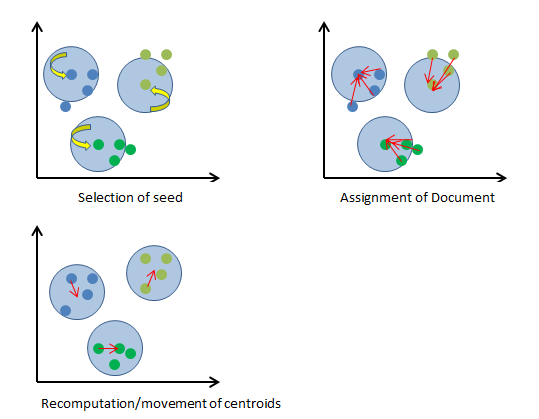
\includegraphics[scale=0.3]{images/kmeans.png}
                            \caption{Source: codeproject.com}
                        \end{figure}
                    }
                \end{block}
            \end{frame}
            \begin{frame}
                \frametitle{Implémentation}
                \only<-7>{
                    Spécificités:
                    \begin{itemize}
                        \pause[2]
                    \item Langage: \pause[3] Java
                        \pause[4]
                        \item Stockage: \pause[5] Annulé
                        \pause[6]
                        \item Utilisation: \pause[7] "Librairie"
                    \end{itemize}
                    \pause[8]
                }
                \only<8>{
                    \begin{block}{Diagramme de classes}
                        \begin{center}
                            \includegraphics[scale=0.1]{graph/v2class.png}
                        \end{center}
                    \end{block}
                    \pause[9]
                }
                \only<9>{
                    \begin{block}{Diagramme de classes}
                        \begin{center}
                            \includegraphics[scale=0.2]{graph/v2classneat.png}
                        \end{center}
                    \end{block}
                }
            \end{frame}
        \subsection{v3 Stockage}
            \begin{frame}
                \frametitle{Problématiques}
                Version Stockage 
                \pause
                \begin{itemize}
                    \item Comment stocker efficacement l'ensemble des données du programme?
                    \pause
                    \item Comment visualiser de manière plus intuitive les données?
                \end{itemize}
            \end{frame}
            \begin{frame}
                \frametitle{Différentes solutions de stockage}
                Deux grandes solutions:
                \pause
                \begin{columns}
                    \begin{column}{4cm}
                        \begin{block}{}
                        \end{block}
                    \end{column}
                \end{columns}
            \end{frame}

    \section{Conclusion}
        \begin{frame}
        \end{frame}
\end{document}
